\documentclass[a4paper, 10pt]{article}

\usepackage[utf8]{inputenc}

%\usepackage[ngerman]{babel}

\usepackage[T1]{fontenc}
\usepackage{amsmath}
\usepackage{graphicx}

\title{Pflichtenheft}
\author{Auftraggeber: Ann-Cathrin Weger, Merten Nagel, Dennis Eylmanns (Gruppe 8) \and
Auftragnehmer: Niklas Adams, David Südholt, Felix Kibellus(Gruppe 6)}
\date{14.10.2014}

\begin{document}
	\maketitle

\section{Zielbestimmungen}
\subsection{Musskriterien}
\begin{enumerate}
\item
Es muss die Evolution einer Spezies in einer zuvor gewählten Welt simuliert werden
\item
Es sollen mindestens vier zuvor generierte Welten zur Auswahl stehen
\item
Zu Beginn der Simulation wird die Spezies erstellt. Dazu steht eine Auswahl rudimentärer Merkmale zur Verfügung, die im Laufe der Simulation ausgeprägt und verfeinert werden können.
\item
Zu einem späteren Zeitpunkt der Simulation sollen konkurrierende Spezies auftreten
\item
Ausrottung der Konkurrenz bzw. das Erlangen der Vormachtstellung kann durch physische oder intellektuelle Überlegenheit erreicht werden. Dies beendet die Simulation
\end{enumerate}

\subsection{Wunschkriterien}
\begin{enumerate}
\item
Welten sollen auch zufällig generiert werden können
\item
Mit anderen Spezies können auch gegenseitig nützliche Beziehung eingegangen werden
\end{enumerate} 

\subsection{Abgrenzungskriterien}
\begin{enumerate}
\item
Der Benutzer greift nur indirekt in die Entwicklung seiner Spezies ein, indem er über Ausprägung von Merkmalen und Fähigkeiten entscheidet. Direkte Steuerung der Individuen ist nicht vorgesehen
\item
Eventuell sollen vernetzte Geräte an derselben Simulation teilnehmen, wobei jede Instanz eine Spezies kontrolliert
\end{enumerate}

\section{Produkteinsatz}
\subsection{Anwendungsbereiche}
Die Simulation ist eher zu Lern- als zu Forschungszwecken einzusetzen
\subsection{Zielgruppen}
\begin{enumerate}
\item Die Software richtet sich an interessierte Laien
\item Die Simulation soll somit eine spielerische Einführung an die Prinzipien der Evolution bieten
\end{enumerate}

\subsection{Betriebsbedingungen}
\subsubsection{Qualifikationsniveau des Benutzers}
Der typische Benutzer verfügt über wenig bis kein fundiertes Fachwissen über die Evolutionstheorie, ist jedoch komfortabel im Umgang mit Technologie
\subsubsection{Betriebsbedingungen des Produktes}
Um die Simulation unabhängig vom Aufenthaltsort des Benutzers überwachen zu können, wird die Software als App für das mobile Betriebssystem Android konzipiert. Unterstützung wird nur für Versionen nach Android 4.0.2 (Ice Cream Sandwich) garantiert.

\section{Produktübersicht}
\begin{enumerate}
\item
Die Simulation läuft auf dem Android-Endgerät des Benutzers
\item
Das Framework zur Betreibung der Applikation, darunter Java VM und graphische Bedienelemente, werden somit von Google bereitgestellt.
\item
Grundsätzlich ist keine Netzwerkverbindung zum Betreiben der Software vonnöten. Es besteht allerdings die Möglichkeit zur Vernetzung und gemeinsamen Simulation mit anderen Geräten.
\end{enumerate}

\section{Produktfunktionen}
\begin{enumerate}
\item[(F01)] Die graphische Oberfläche wird für das Android-Betriebssystem entworfen und benutzt das von Google bereitgestellte Java-Framework. 

\item[(F02)] Es soll einen Startbildschirm geben, welcher dem Benutzer beim Programmstart angezeigt wird.
\begin{enumerate}
\item[(F02.1)]
Der Benutzer kann sich eine Erklärung des Simulators in Textform anzeigen lassen. Dies soll jedoch nur eine kleine Hilfestellung sein, da der Simulator intuitiv und selbsterklärend aufgebaut sein wird.
\item[(F02.2)]
Es soll einen Button geben, mit welchem der Benutzer die Simulation starten kann.
\item[(F02.3)]
Der Benutzer soll die Möglichkeit haben unterbrochene Simulationen zu laden.
\item[(F02.4)]
Es soll einen Button geben, mit welchem der Benutzer die vergangenen Simulationen anzeigen lassen kann.
\item[(F02.5)]
Über den "Zurück-Button" kann das Programm beendet werden.
\end{enumerate}


\item[(F03)]
Der Benutzer hat die Möglichkeit aus einer festgelegten Menge vordefinierter Welten zu wählen um eine Simulation unter gleichen Bedingungen erneut durchzuführen.
Es steht auch die Möglichkeit zur Verfügung eine Simulation auf einer neu generierten Welt vorzunehmen.
Beim generieren der Welt werden größere Gebiete der gleichen Eigenschaft erstellt. Unterschiedliche Landbereiche haben unterschiedliche Eigenschaften.

\item[(F04)]
Erstellen einer eigenen Spezies
\begin{enumerate}
\item[(F04.1)]
Dem Benutzer wird ein Textfeld zur Benennung der Spezies zur Verfügung gestellt
\item[(F04.2)] Spezifizierbare Eigenschaften der Spezies
\begin{enumerate}
\item[(F04.2.1)]
Zu Beginn wird der Nutzer vor die Wahl zwischen gewissen Grundeigenschaften gestellt, darunter Art der Nahrungsaufnahme (Fleischfresser, Pflanzenfresser), Lebensraum (Land, Wasser, Luft), Lebensweise (Rudeltier, Einzelgänger) u.a.
\item[(F04.2.2)]
Diese beeinflussen die fünf Kernattribute der Spezies: Physische Kraft, Geschicklichkeit, Intelligenz, soziale Kompetenz sowie Fortpflanzungsrate (inklusive Überlebensfähigkeit der Jungen)
\item[(F04.2.3)]
Im Verlauf der Simulation erhält der Benutzer Punkte, die von der Größe seiner Population abhängt
\item[(F04.2.4)]
Der Benutzer kann diese Punkte in einen Merkmalsbaum und einen Fähigkeitenbaum investieren, um seine Spezies zu entwickeln.
\item[(F04.2.5)]
Der Merkmalsbaum enthält physische Charakteristika wie Gliedmaßen, Sinnesorgane etc.
\item[(F04.2.6)]
Der Fähigkeitenbaum enthält Fähigkeiten, deren Erlernbarkeit von den bereits ausgebildeten Merkmalen und Kernattributen abhängt. Beispielsweise hängt die Fähigkeit, Feuer zu machen, von dem Kernattribut Geschicklichkeit und der physischen Charakteristik Hände ab.
\item[(F04.2.7)]
Die in den Bäumen verteilten Punkte beeinflussen die Kernattribute, Ausbreitung und Fortbestand der Spezies, im Besonderen in der Interaktion mit anderen Spezies.
\end{enumerate}

\item[(F04.3)]
Bei Bestätigung der Konfiguration durch den Benutzer wird die Spezies gespeichert und die Simulation gestartet.
\end{enumerate}

\item[(F05)]
Der Startort wird, abhängig von den gewählten Grundeigenschaften, zufällig auf der Karte festgelegt. Der Bereich, an dem die Spezies startet, wird aufgedeckt, der anfangs verdeckten Rest der Karte kann durch Besiedelung erkundet werden.


\item[(L06)]
Der Benutzer startet im Jahre 0. Eine Minute in Echtzeit entspricht 100.000 Jahren in der Simulation. Somit entspricht eine durchschnittliche Simulation (20 Minuten) 20.000.000 Jahren Evolution.
 
\item[(L07)]
Die Erweiterungen und Veränderungen der Spezies wurden schon genauer in (L04) spezifiziert um die Erstellung der Spezies besser mit der Entwicklung in Verbindung zu setzen und zu erklären. Die Speicherung der Inhalte geschieht sobald sich der Datenbestand geändert hat. Sollte die Simulation unterbrochen werden oder abstürzen gehen keine Daten verloren. 

\item[(L08)]
Sollte eine andere Spezies vernichtet werden, so erscheint dem Benutzer ein kleines Dialogfenster, welches durch einen Button "Schließen" zu beenden ist. 

\item[(L09)]
Bei Negativereignissen bezüglich der eigenen Spezies soll ebenfalls ein Dialogfenster informieren. Dies ist der Fall, wenn das Wachstum der eigenen Spezies negativ wird oder die eigene Spezies kurz vor der Ausrottung steht.


\item[(L10)]
Es können verschiedene Zufallsereignisse auftreten
\begin{enumerate}
\item[(L10.1))]
Eiszeit
\item[(L10.2))]
Klimaerwärmung
\item[(L10.3))]
Meteoriteneinschlag auf ein Gebiet, welches nahezu die gesamte dort lebende Spezies ausrottet. 
\item[(L10.4))]
Erhöhte Radioaktive Belastung über kurzen Zeitraum
In einem Gebiet sterben einige Individuen an der erhöhten Strahlung. Die anderen generieren zusätzliche Mutationspunkte, da es durch der Strahlung zu Mutationen kam.

\end{enumerate}


\item[(L11)]
Der Benutzer kann die Simulation jederzeit vorzeitig beenden. In diesem Fall erscheint ein Dialogfenster, in dem der Benutzer entscheiden kann, ob die derzeitige Simulation gespeichert werden soll. Möchte der Benutzer nicht speichert, werden alle zu der Simulation gehörigen Daten gelöscht.

\item[(L12)]
Beim natürlichen Ende der Simulation wird dem Benutzer eine Statistik Angezeigt. Diese enthält die Simulationszeit, die derzeitige Populationsgröße, die 5 Kernattribute und eine Wertung.

\end{enumerate}

\section{Produktdaten}
\begin{enumerate}
\item[(D01)]
Es fallen lediglich Einstellungsdaten und Simulationsdaten an
\begin{enumerate}
\item[(D01.1)]
Wird de Simulation unterbrochen, werden die Populationsbestände, die Evolutionspunkte und die derzeitige Entwicklung jeder Spezies gespeichert.
\item[(D01.2)]
Wird die Simulation vorzeitig beendet, so wird nichts gespeichert.
Wird die Simulation abgeschlossen werden die in (L12) spezifizierten Daten abgespeichert.
\end{enumerate}
\end{enumerate}

\section{Produktleistungen}
Die Zeit wird sekündlich aktualisiert und in die Evolutionszeit umgerechnet. Die Umrechnung wurde bereits in (L06) spezifiziert.

\section{Qualitätsanforderungen}
Der Benutzer hat jederzeit die Möglichkeit alle relevanten Daten der Spezies, welche direkt von ihm manipuliert werden können einzusehen. Die Ansicht der Kernattribute erfolgt über ein Balkendiagramm. Implementierungsspezifische Variablenwerte bleiben jedoch verborgen.

\section{Benutzungsoberfläche}
Die wichtigsten Darstellungsfenster sind
\begin{enumerate}
\item[(B01)] Startbildschirm
\item[(B02)] Weltenauswahl
\item[(B03)] Simulations- und Weltansicht
\item[(B04)] Weiterentwicklungsansicht
\item[(B05)] Information über die verschiedenen Spezies
\end{enumerate}
Die genaue Darstellung geht aus den folgenden Bildern hervor.

\begin{minipage}{49mm} 
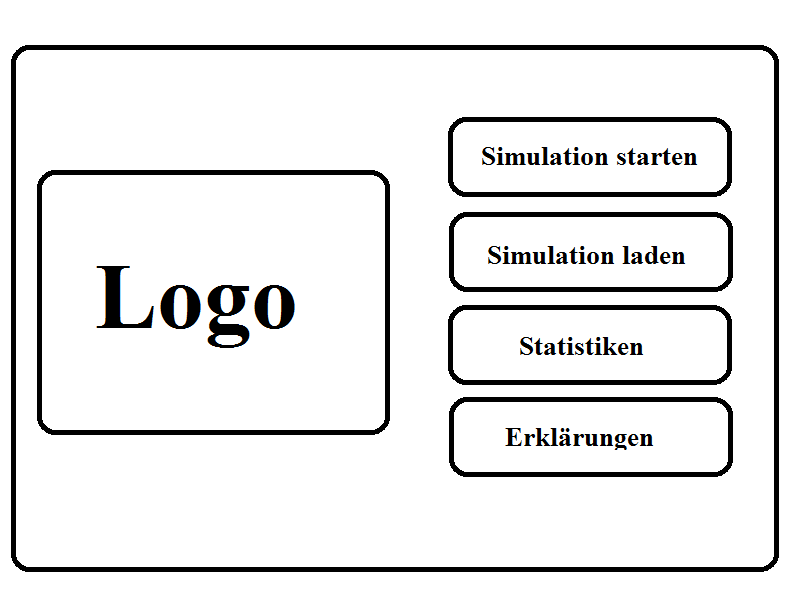
\includegraphics[scale=0.45]{Bilder/Startbildschirm.png}
Startbildschirm
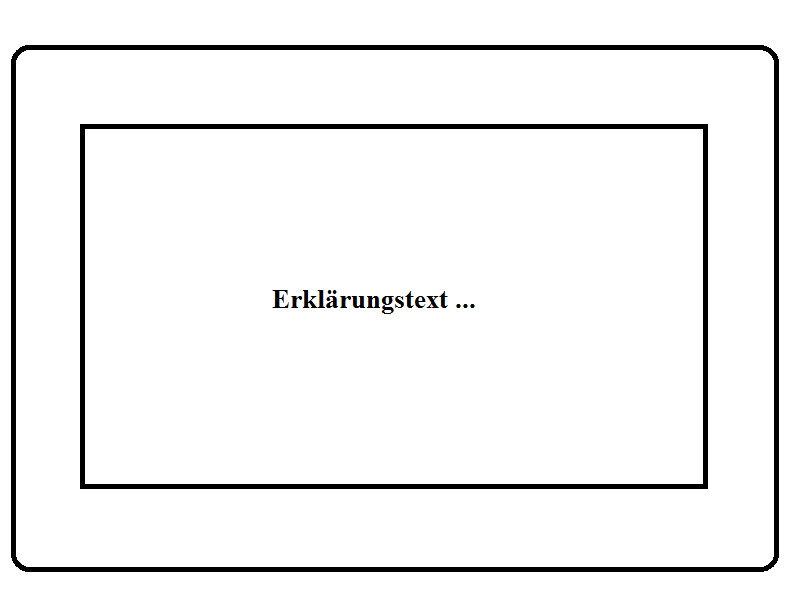
\includegraphics[scale=0.45]{Bilder/Erklarungstext.png}
Erklärungstext
\end{minipage}

\begin{minipage}{49mm} 
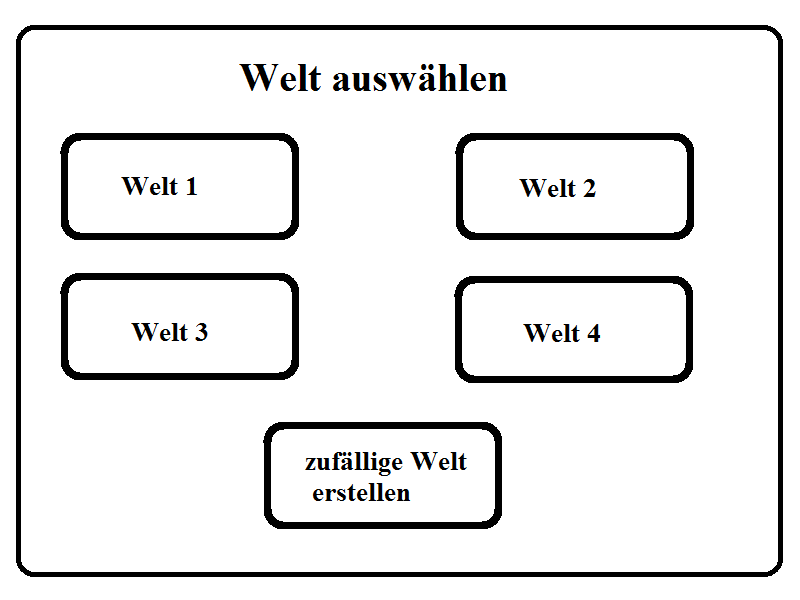
\includegraphics[scale=0.45]{Bilder/WeltWahl.png}
Weltauswahl
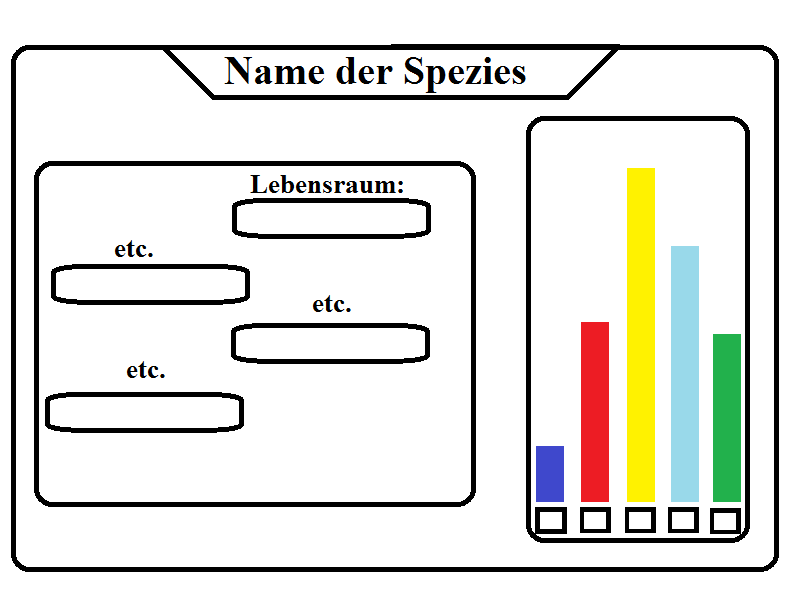
\includegraphics[scale=0.45]{Bilder/Spezies_Erstellen.png}
Spezieskreation
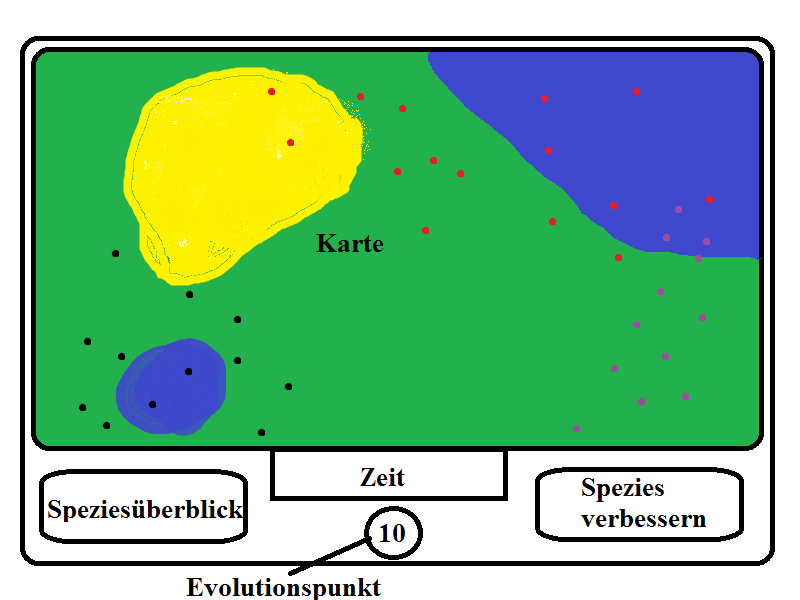
\includegraphics[scale=0.45]{Bilder/Simulationsbildschirm.png}
Simulationsanzeige
\end{minipage}

\begin{minipage}{49mm} 
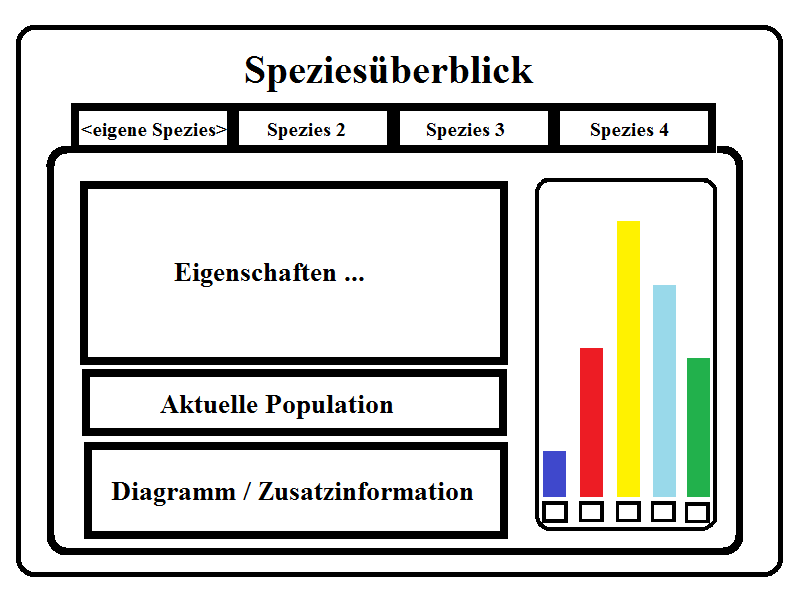
\includegraphics[scale=0.45]{Bilder/Speziesuberblick.png}
Speziesüberblick
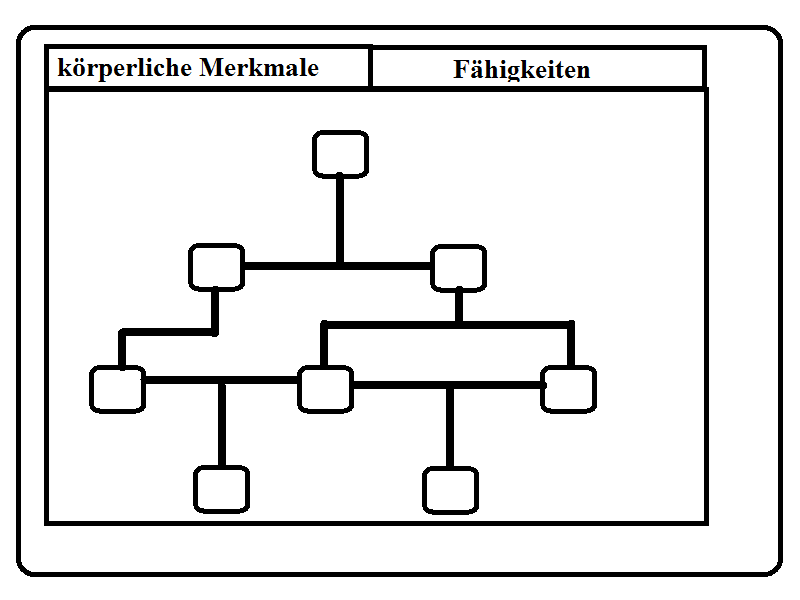
\includegraphics[scale=0.45]{Bilder/Fahigkeiten.png}
Spezies weiterentwickeln
\end{minipage}



\section{Nichtfunktionale Anforderungen}
Das Programm soll zuverlässig und stabil arbeiten.
Falls die Simulation doch einmal abstürzen sollte die Daten wiederherstellbar sein, sodass die Simulation fortgesetzt werden kann. Die Simulation soll keine exakte Wissenschaftliche Nachbildung sein, sich jedoch stark daran orientieren. Die flüchtigen Daten sollen nicht mehr Speicherplatz als 1 GB benötigen. Die persistenten Daten können abhängig von der Anzahl der gespeicherten Simulationen stark variieren. Die Darstellung der graphischen Inhalte soll auf jedem Android-Endgerät gleich proportioniert sein.
Das Programm soll jederzeit effizient arbeiten und der Benutzer soll nicht das Gefühl haben auf das Programm warten zu müssen. Die Basissimulation soll nicht vom Zielsystem abhängen und die Benutzeroberfläche soll leicht auszutauschen sein um eine optimale Portierbarkeit zu gewährleisten.

\section{Technische Produktumgebung}
\subsection{Software}
Auf dem Endgerät muss das Betriebssystem Android laufen.
\subsection{Hardware}
Minimalanforderungen für die Hardware sind:
\begin{enumerate}
\item CPU:1GHz single Core
\item RAM: 512 MB
\item verfügbarer interner Speicher: 1GB 
\item Touchscreen
\end{enumerate}
\subsection{Orgware}
Es wird keine zusätzliche Orgware benötigt.
\subsection{Produktschnittstellen}
Auf der Ansichtsebene wird eng mit Android zusammengearbeitet. 

\section{Spezielle Anforderungen an die Entwicklungsumgebung}
\subsection{Software}
Entwickelt wird unter einem Linux-Betriebssystem.
Zur Versionsverwaltung wird Git verwendet.
Zur Generierung der Anwendung wird Ant verwendet.
Als Entwicklungsumgebung wird Eclipse mit installiertem Android-SDK verwendet. (Android Development Tool)
Zum Testen wird das Betriebssystem Android verwendet.
Mit ObjectAid und yEd werden UML-Diagramme generiert.

\subsection{Hardware}
Zum Testen werden Endgeräte verwendet, welche die in 10.2 aufgeführten Minimalanforderungen erfüllen. Zur Entwicklung werden die am Arbeitsplatz bereitgestellten Rechner und private Geräte verwendet.

\subsection{Orgware}
Zu Planungszwecken wird innerhalb des Git-Repositories eine Liste mit noch zu erledigenden Aufgaben geführt.
Zu Dokumentationszwecken findet sich dort ebenfalls eine Liste in der bereits erledigte Aufgaben dokumentiert werden, um später den Entwicklungsprozess nachvollziehen zu können. Ergebnisse der Planungsphase wie beispielsweise UML-Diagramme werden ebenfalls archiviert, sodass diese jederzeit von allen Entwicklern einsehbar sind.
\subsection{Entwicklungsschnittstellen}
Das Programm ist grob in folgende Module zu unterteilen:
\begin{enumerate}
\item graphische Oberfläche
\item eigentliche Simulation (mathematische Berechnungen)
\item Generierungsalgorithmen
\item künstliche Intelligenz 
\item Datenhaltung
\end{enumerate}

\section{Gliederung in Teilprodukte}
\subsection{Simulationsentwicklung}
Zu Beginn soll nur das von der GUI abgekapselte Simulationsmodell erstellt werden.
\subsection{GUI-Verknüpfung}
Die Simulations wird mit Android verknüpft und so benutzbar gemacht.
\subsection{Mehrbenutzer über Netzwerk}
Durch ein Mehrbenutzersystem auf unterschiedlichen Geräten wird die Simulation nun für mehrere Benutzer parallel benutzbar gemacht.

\section{Ergänzungen}
Das Programm soll wie üblich vom Android-Betriebssystem installierbar sein.

\end{document}